%% The following is a directive for TeXShop to indicate the main file
%%!TEX root = main.tex

% ===========================================================================================
\chapter{\textbf{Evaluation of \ac{CORGIDS}}}
\label{sec6:Evaluation}
In this chapter, the results from the sensitivity analysis and attacks seeded in ~\autoref{ch:Attacks} are presented. Also, additional experiments which provide more insight about how the tuning parameters of the trained HMM from phase two of workflow of \ac{CORGIDS} (\autoref{sec3:Approach}), effect the precision and recall were performed. The motive behind discussing the results achieved by \ac{CORGIDS} is to measure its performance in terms of the evaluation criteria described in this chapter.

\section{Sensitivity Analysis}
\label{sensitivityAnalysis}

Before evaluating \ac{CORGIDS}, a sensitivity analysis to find out the values of the three experimental parameters was performed. Sensitivity analysis is a study which determines how different values of an independent variable affect a particular dependent variable under a given set of assumptions. It can be used within given boundaries that depend on one or more input variables, such as the effect that changes in interest rates has on bond prices. The three experimental parameters for which the sensitivity analysis was carried out are as follows.

\begin{itemize}
\item Window size (\textit{w}): A window size is defined as the time duration which is under consideration for detecting an intrusion~\cite{zohrevand2016hidden} in a \ac{SUT}. A large \textit{w} means that greater historical data is given to the \ac{HMM} to decide of a malicious activity.
\item Acceptable range ($\delta$): An acceptable range defines a range within which the testing system trace's likelihood can vary from the mean log likelihood from the trained \ac{HMM}. A testing trace with the value within range from the specified mean will be marked to be similar to the training traces. If the value of $\delta$ is chosen to be large, it means that there is enforcement of loose control and allowing system traces with substantial variation from the trained \ac{HMM} to be considered benign.
\item Threshold of consecutive decisions ($\lambda$): Stateful tests~\cite{urbina2016limiting} are performed by maintaining the historical decisions of the \ac{IDS} and generating alert only if it goes above a chosen threshold. The intuition behind using the $\lambda$ is to look back at the historical decisions of the intrusion detector to see if there is really an anomaly or if it is just one time spike in the system. Greater value of $\lambda$ enforces more number of consecutive historical intrusion decisions to generate an alert.
\end{itemize}

The values of \textit{w}, $\delta$ and $\lambda$ were chosen based on the highest values of precision and recall (\autoref{sec:metrics}) achieved in this experiment. The results from sensitivity analysis are shown in ~\autoref{fig:sensitivityAnalysis}, ~\autoref{fig:sensitivityAnalysis_2} and ~\autoref{fig:sensitivityAnalysis_3}. \textit{w} is measured in minutes while $\delta$ in standard deviations. A key point to note here is that more the value of precision and recall for a set of experimental parameters, higher is the rate of detection. This experiment was carried out by varying one parameter at a time and keeping others constant. For instance, graph \textit{a} in ~\autoref{fig:sensitivityAnalysis} denotes the scenario where the \textit{w} is varied from 2 to 4 minutes while keeping $\delta$ = 1 and $\lambda$ = 2. Following similar pattern from  graph \textit{a}, the constant parameters will be swept , that is, $\delta$ and $\lambda$ from their lowest to the highest values. This forms the graphs \textit{a} - \textit{d} in ~\autoref{fig:sensitivityAnalysis}. Therefore, similar to ~\autoref{fig:sensitivityAnalysis}, other experiments were conducted by varying $\delta$ in ~\autoref{fig:sensitivityAnalysis_2} and $\lambda$ in ~\autoref{fig:sensitivityAnalysis_3}. This sensitivity analysis represents the data collected from the distance spoofing attack on the \ac{UAV} testbed. 
%Though similar analysis was performed for the other attacks on the \ac{UAV} and \ac{SAP}, due to space limitations they are not included here. 

From the graphs, it can be seen that the precision and recall are increasing as the \textit{w} is increasing from 2 to 4 minutes, while they are decreasing when the $\delta$ and $\lambda$ are increasing from 1 to 3 standard deviations and 2 to 4 decisions respectively. From this trend it can be inferred that the precision and recall are largest when the \textit{w} is large with small $\lambda$ and $\delta$. Similar trend was observed for other attacks on the two test-beds. The reason for the trend that was observed is that a \ac{HMM} requires substantial historical data to determine if there is some anomaly in the system. With lesser history (smaller window size), it is unable to correctly infer the current state of the system. Therefore, when a greater \textit{w} of 4 minutes is provided, it is able to create a more realistic model of the system, as the \ac{HMM} is now more behaviorally knowledgeable about the system after having a large \textit{w} and can now make decisions with higher likelihood, thus giving the best results for the least value of $\delta$ and $\lambda$.


An important point to note here is that though \ac{CORGIDS} is able to detect attacks even with less favorable values of \textit{w}, $\lambda$ and $\delta$, it achieves less precision and recall in doing so. On the other hand, if the results obtained from sensitivity analysis are used, higher values of precision and recall can be achieved. Therefore, either the lesser favorable parameters can be chosen and results can be obtained quickly at the cost of accuracy, or with the most favorable parameters, fewer \ac{FN} can be obtained, while incurring some latency.


\begin{figure}%
    \centering
    \subfloat[$\delta$ = 1 and $\lambda$ = 2]{{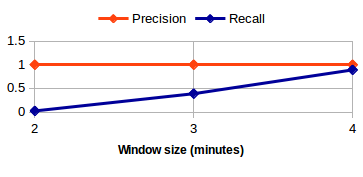
\includegraphics[width=0.50\textwidth]{Graphics/Spoofing_Window_1.png} }}%
    \subfloat[$\delta$ = 3 and $\lambda$ = 2]{{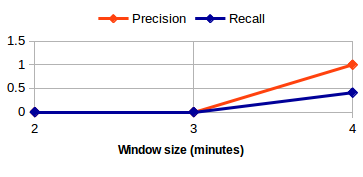
\includegraphics[width=0.50\textwidth]{Graphics/Spoofing_Window_2.png} }}%
    \qquad
    \subfloat[$\delta$ = 1 and $\lambda$ = 4]{{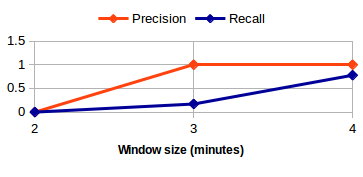
\includegraphics[width=0.50\textwidth]{Graphics/Spoofing_Window_3.png} }}%
    \subfloat[$\delta$ = 3 and $\lambda$ = 4]{{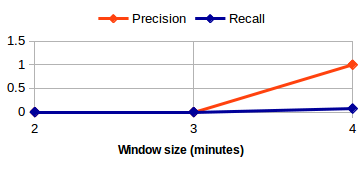
\includegraphics[width=0.50\textwidth]{Graphics/Spoofing_Window_4.png} }}%
    \caption{Sensitivity Analysis: Independent variables are $\delta$ and $\lambda$. Dependent variable is \textit{w}. The vertical axes in all figures are the values of precision and recall calculated after averaging 5 fold cross validation of test system traces.}%
    \label{fig:sensitivityAnalysis}%
\end{figure}

\begin{figure}
    \centering
    \subfloat[\textit{w} = 2 and $\lambda$ = 2]{{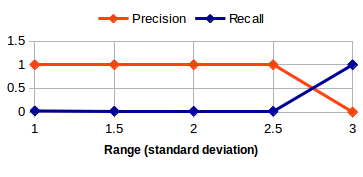
\includegraphics[width=0.50\textwidth]{Graphics/Spoofing_Range_1.png} }}%
    \subfloat[\textit{w} = 4 and $\lambda$ = 2]{{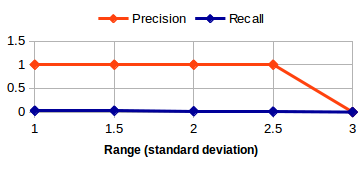
\includegraphics[width=0.50\textwidth]{Graphics/Spoofing_Range_2.png} }}%
    \qquad
    \subfloat[\textit{w} = 2 and $\lambda$ = 4]{{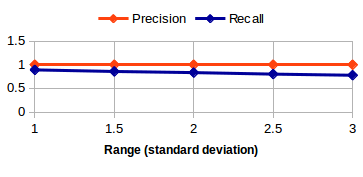
\includegraphics[width=0.50\textwidth]{Graphics/Spoofing_Range_3.png} }}%
    \subfloat[\textit{w} = 4 and $\lambda$ = 4]{{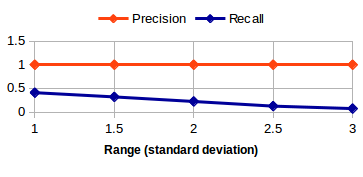
\includegraphics[width=0.50\textwidth]{Graphics/Spoofing_Range_4.png} }}%
    \caption{Sensitivity Analysis: Independent variables are \textit{w} and $\lambda$. Dependent variable is $\delta$. The vertical axes in all figures are the values of precision and recall calculated after averaging 5 fold cross validation of test system traces.}%
    \label{fig:sensitivityAnalysis_2}%
\end{figure}

\begin{figure}%
    \centering
    \subfloat[\textit{w} = 2 and $\delta$ = 1]{{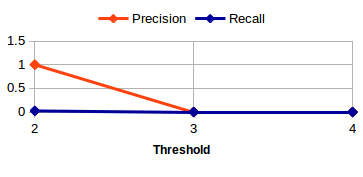
\includegraphics[width=0.50\textwidth]{Graphics/Spoofing_Decision_1.png} }}%
    \subfloat[\textit{w} = 2 and $\delta$ = 3]{{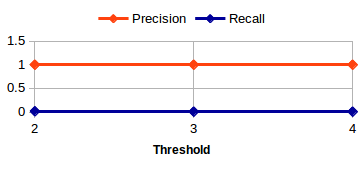
\includegraphics[width=0.50\textwidth]{Graphics/Spoofing_Decision_2.png} }}%
    \qquad
    \subfloat[\textit{w} = 4 and $\delta$ = 1]{{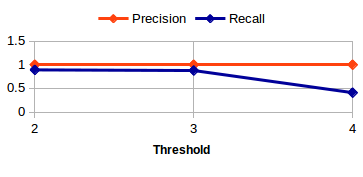
\includegraphics[width=0.50\textwidth]{Graphics/Spoofing_Decision_3.png} }}%
    \subfloat[\textit{w} = 4 and $\delta$ = 3]{{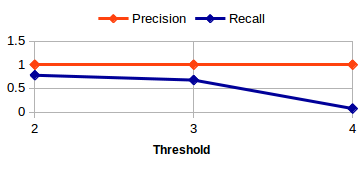
\includegraphics[width=0.50\textwidth]{Graphics/Spoofing_Decision_4.png} }}%
    \caption{Sensitivity Analysis: Independent variables are \textit{w} and $\delta$. Dependent variable is $\lambda$. The vertical axes in all figures are the values of precision and recall calculated after averaging 5 fold cross validation of test system traces.}%
    \label{fig:sensitivityAnalysis_3}%
\end{figure}

\section{Evaluation Criteria}
\label{sec:metrics}

Precision, recall, \ac{FP}, \ac{FN}, performance overheads and memory overheads were used to evaluate \ac{CORGIDS}. These metrics are explained below:

\begin{itemize}
\item Precision: For a malicious execution of \ac{SUT}, when an intrusion detector correctly detects an intrusion, is called precision. For an intrusion detector, the higher precision the better.
\item Recall: On the other hand, recall is the percentage when the \ac{SUT} execution was malicious and the intrusion detector correctly identified it among all the malicious \ac{SUT} executions. For an intrusion detector, the higher recall the better.
\item \acf{FP}: Represents the ratio of execution traces that were falsely reported as malicious to the total number of normal traces for a given \ac{CPS}.
\item \acf{FN}: Represents the ratio of malicious attacks that went undetected/unnoticed by the IDS to the total number of attacks for a given \ac{CPS}.
\item Performance Overhead: Performance overhead reflects the additional time taken, when \ac{CORGIDS} is deployed on the \ac{SUT}. It helps to determine if the time taken by the \ac{IDS} to detect intrusion is greater than the time taken to complete a closed loop once, in which case it is not very helpful to use an \ac{IDS}.
\item Memory Overhead: As the devices in which \ac{CORGIDS} will be used will be memory constrained, it is essential to calculate its memory overhead. Memory occupied by \ac{CORGIDS} on \ac{SUT} will be used to determine this overhead.
\end{itemize}

%As there wasn't a real \ac{UAV} and a simulator was used for the \ac{UAV} experiments, and therefore memory and performance overheads for \ac{UAV} test-bed were not calculated.

\begin{table}
\centering
  \caption{False Positive and False Negative obtained for CORGIDS on the two test-beds}
  \label{tab:results}
  \scalebox{0.9}{
  \begin{tabular}{|c|c|c|l|}
    \toprule
    \textbf{Testbed}&\textbf{Targeted Attack}&\textbf{FP (\%)}&\textbf{FN(\%)}\\
    \midrule
    \multirow{3}{*}{UAV}& Battery Tampering&0.0&12.20\\
                        & Flooding&0.0&11.30\\
                        & Distance Spoofing&0.0&12.80\\
    \hline
    \multirow{2}{*}{SAP}& Insulin Tampering&5.60&4.20\\
                            & Glucose Spoofing&2.80&8.40\\
    \hline
\end{tabular}
}
\end{table}


\begin{table}
\centering
  \caption{Comparison of Precision and Recall for OpenAPS platform}
  \label{tab:comparisonOfResults}
  \scalebox{0.9}{
  \begin{tabular}{|p{2.2cm}|p{2.0cm}|p{1.0cm}|p{1.0cm}|p{2.0cm}|p{1.8cm}|}
    \toprule
    \textbf{Methodology}&\textbf{Testbed}&\textbf{FP(\%)}&\textbf{FN(\%)}&\textbf{Precision(\%)}&\textbf{Recall(\%)}\\
    \midrule
    \multirow{2}{*}{ARTINALI}& SEGMeter&12&2.3&89.06&97.7\\
                        & OpenAPS&13.5&2&87.89&98\\

    \hline
    Zohrevand&Water&&& &\\
    et al.~\cite{zohrevand2016hidden}&Treatment&- &- & 78.87&81.4\\
     & System& & & & \\
    \hline
    Chen &Water &&&&\\
    et al.~\cite{chen2018learning}&Purification &- &15 &- &- \\
     &Plant& & & & \\
    \hline
    \multirow{2}{*}{CORGIDS}& UAV&0.00&12.10&100&87.90\\
                            & SAP&4.20&6.30&95.70&93.70\\

    \hline
\end{tabular}
}
\end{table}

For evaluating \ac{CORGIDS}, the value obtained for each of the three variables (\textit{w}, $\lambda$ and $\delta$) from the sensitivity analysis was used. ~\autoref{tab:results} contains the results for \ac{FP} and \ac{FN} for the two test-beds, namely, an \ac{UAV} and \ac{SAP} on which \ac{CORGIDS} was deployed. ~\autoref{tab:comparisonOfResults} compares our results to only those related papers~\cite{chen2018learning,zohrevand2016hidden,aliabadi2017artinali} which dynamically generate physical invariants \footnote{Note: For the research papers that were used for comparison with \ac{CORGIDS} for the \ac{UAV} and \ac{SAP} test-bed, the \ac{FP}, \ac{FN}, precision and recall values were directly used. Manual calculation of precision and recall for~\cite{aliabadi2017artinali} was made from the \ac{FP} and \ac{FN} values provided in their paper.}. We acknowledge that ~\autoref{tab:comparisonOfResults} does not provide a complete comparison as the test-beds, attacks and training and testing scenarios were different for each \ac{IDS}, however we include it here to provide better context about \ac{CORGIDS} performance. Later in ~\autoref{ch:comparisonwithrelatedwork}, a comprehensive comparison of CORGIDS with its related work is described.

Krotofil et. al. and Iturbe et. al.~\cite{krotofil2015process,iturbe2017feasibility} do not measure the performance of their methodology, and hence they could not be compared with \ac{CORGIDS}. In addition, precision and recall for \ac{CORGIDS} and the papers mentioned in ~\autoref{tab:comparisonOfResults} were calculated. To calculate the \ac{FP} and \ac{FN} values for \ac{CORGIDS} which will be used to generate precision and recall, \ac{FP} and \ac{FN} values from ~\autoref{tab:results} were averaged. However, comparison of the precision value of \ac{CORGIDS} with Chen et. al.~\cite{chen2018learning} could not be made, as the later did not provide it in their paper.  

\section{Experiment results} 
Based on the above described metrics, we now discuss the results of the experiments performed.

\subsection{Precision}
In this subsection, the precision achieved by seeding the attacks on the \ac{SUT} and using \ac{CORGIDS} to detect an intrusion is discussed. Also,  the precision achieved with prior work in  ~\autoref{tab:comparisonOfResults} is shown. As can be observed, \ac{CORGIDS} achieves a precision of 100\% and 95.70\% for the \ac{UAV} and \ac{SAP} platform respectively. In comparison, no other intrusion detector has a precision greater than 90\%. Specifically, \ac{CORGIDS} provides an 21.33\% improvement in precision over Zohravend et al. \cite{zohrevand2016hidden} and approximately 8.88\% over Aliabadi et al. \cite{aliabadi2017artinali} for the \ac{SAP} platform.

The reason behind the higher precision percentage for \ac{CORGIDS} is the use of correlations exhibited by the two CPS. \ac{CORGIDS} detects attacks by using an \ac{HMM} to infer if the current system trace exhibits the same trend with which it was trained. This is the reason that especially for the \ac{UAV} platform, the \ac{HMM} recognizes an anomaly with almost 100\% precision. The reason for comparatively low precision value for \ac{SAP} platform is the lack of traces. As the total number of traces for the \ac{SAP} platform were less, it led to even lower training traces, which eventually effected the modeling of the \ac{HMM}. For the experiments on both the test-beds, 70\%:30\% ratio for training and testing traces was maintained. However, the lack of availability of patient's diabetic therapy data led to a lower number of training traces. This, in turn negatively affected the training of the \ac{HMM} used by \ac{CORGIDS} for the \ac{SAP} platform.

\subsection{Recall}
The recall factor of \ac{CORGIDS} is discussed here and compared to the related work mentioned in ~\autoref{tab:results} and ~\autoref{tab:comparisonOfResults} respectively. From  ~\autoref{tab:comparisonOfResults}, it can be observed that \ac{CORGIDS} receives a high recall percentage among all the related work. Although, \ac{CORGIDS} does not have the highest recall, it is quite close to ARTINALI with 93.70\% for the \ac{SAP} platform. \ac{CORGIDS} improves the recall by 15.11\% when compared to  Zohravend et al.~\cite{zohrevand2016hidden}. On the other hand, \ac{CORGIDS} achieves 11.14\% lower recall than ARTINALI when both of them are compared with their lowest recall factors. 

 
\ac{CORGIDS} achieves lesser recall than ARTINALI~\cite{aliabadi2017artinali} mainly because the behavior of the \ac{SUT} under attack was stealthy and did not deviate much from the normal trend. As the deviation was less, the logical correlation between the properties seemed very similar to the one expected, thus the \ac{HMM} did not mark the state as anomalous, leading to some false-negatives. Chen et al. ~\cite{chen2018learning} do not provide recall factor, but give the value of \ac{FN} for their approach, the \ac{FN} value is compared to \ac{CORGIDS}, which is 15\%. This is higher than \ac{CORGIDS} \ac{FN} values of 12.10\% and 6.30\% for the two platforms. Chen et al. use \ac{SVM} for intrusion detection, while \ac{CORGIDS} uses \ac{HMM}. \ac{HMM} are able to better capture the sequence of states and their transitions in a \ac{CPS}, and hence \ac{CORGIDS} achieves lower \ac{FN} values.

\subsection{Memory overhead}
Measurements of the memory overhead of \ac{CORGIDS} running on the \ac{SAP} platform were also collected. The experiments were performed on a Raspberry Pi 3 with approximately 1 GB of RAM. We found that \ac{CORGIDS} consumes 36.15 MB when detecting intrusion. The reason behind this memory overhead is that \ac{CORGIDS} uses \ac{HMM} for intrusion detection. The trained \ac{HMM} model when loaded into memory along with the libraries required for it to generate a decision, requires more space. However, as \ac{CORGIDS} is used by controller to detect intrusion in the \ac{SUT}, and the controllers are not memory constrained as compared to the \ac{SUT}. For instance, in Raspberry Pi 3, it took only a fraction (36.15 MB) of memory from the 1 GB available RAM. Thus, we surmise that the memory overhead incurred by \ac{CORGIDS} is acceptable.

\subsection{Performance overhead}
Like memory overhead, performance overhead measurements were also taken from the Raspberry Pi 3 platform. The average of 10 executions was considered for the overhead tests.  
Ideally, the time taken to deduce a decision should be less that the execution cycle of the \ac{SUT}, in order for the intrusion detector to keep up with the system. The execution cycle time is the time taken to go though once the closed loop of a \ac{CPS}. The execution cycle time is important because it gives an idea of how much time the system takes to complete one loop of input from blood glucose sensors, to calculating the insulin dosage and sending the same to the insulin pump. It takes approximately 1.25 seconds for \ac{CORGIDS} to generate a decision based on the input correlated logs. This is negligible compared to the time taken by a single execution cycle of \ac{SAP}, which is about 5 minutes.

\bigskip
\textbf{Scalability of CORGIDS:} To understand the scalability of the overheads with \ac{HMM} size, the \ac{HMM} used for intrusion detection were varied. Thus, multiple \ac{HMM} were created by varying the tuning parameter, the number of \textit{hiddenStates}. The number of \textit{hiddenStates} were varied among {2, 5, 10, 15, 20}. We observed that the memory and performance overhead of \ac{CORGIDS} remains the same regardless of the number of \textit{hiddenStates} in the \ac{HMM}. This is could be because the libraries which are loaded along with the \ac{HMM} is the dominant factor in the time, and this does not depend on the number of \textit{hiddenStates} in the \ac{HMM}.

\section{Additional experiments}
We carried out additional experiments to gather more insight about how the \textit{precision} and \textit{recall} vary based on the type of trained \ac{HMM}.
We conduct experiments which include the variation of the two parameters which determine the type of trained \ac{HMM} that will be generated.
\begin{itemize}
\item Training threshold - Training threshold is used as a stopping criteria for training the \ac{HMM} in \textit{Building an Intrusion Detector} phase. This value signifies the maximum difference between current and previous \ac{HMM} log likelihood, if the current \ac{HMM} is the trained \ac{HMM}. We used the value of 0.5\% as the \textit{training threshold} in ~\autoref{sec3:Approach} based on the prior work~\cite{ferrer2000influence}. However, through this experiment we want to determine the effect that the change of this value has on intrusion detection capability of the trained \ac{HMM}. We sweep the value of training threshold from the values (0.35\%, 1\% and 2\%) with 0.5\% value already being used in our experiments.

\item Number of training traces - The number of training traces determine the context that the trained \ac{HMM} will have. Higher the number of training traces, more likely is that the \ac{HMM} will be equipped with different types of behavior exhibited by the \ac{CPS}. For our experiments, we kept the value of training to testing traces to be 70\% : 30\%. However, for this study we varied this ratio to see what effect it had on the precision and recall of the \ac{IDS}. Therefore, the ratio of training traces to testing traces was varied between (50\% : 50\%, 60\% : 40\% and 80\% : 20\%) with 70\% : 30\% ratio already covered in the above experiments.
\end{itemize}

Both parameters - training threshold and number of training traces - discussed above are varied one by one, i.e. while one is varied other is kept constant, and vice-versa. Also, this study was conducted for both the platforms - \ac{UAV} and \ac{SAP}.

\subsection{Additional results for UAV platform}
We conducted two experiments, one for each of the two parameters and summarize the results below.

\begin{itemize}

\item \textit{Training threshold}: By varying the training threshold and keeping the number of training to testing traces constant to 70\% : 30\%, we got the result shown in ~\autoref{fig:UAV_threshold}. Similar trend of precision and recall was observed for each of the individual value of training threshold as when the training threshold was 0.5\%. Also, it was seen that the training threshold did effect the recall factor of \ac{CORGIDS}. It can be seen that the recall increases as the training threshold decrease. So, for 0.35\% as the training threshold we get the maximum value of recall. However, the recall offered by training threshold value of 0.5\% is very close to the maximum recall value achieved in this experiments. Therefore, while using 0.5\% for the attacks which we reported in ~\autoref{ch:Attacks}, we did not sacrifice the intrusion detection capabilities of \ac{CORGIDS} by using an under-trained \ac{HMM}. On the other hand, it can also be seen that the precision remains unaffected by the change in training threshold, this could be because the trained \ac{HMM} which we got from each of the individual experiments was well trained about the benign behavior of the \ac{SUT}.

Another observation we made was that the time taken to get the trained \ac{HMM} model increased as the training threshold decreased. It was because, the maximum difference between the log likelihood's of the two \ac{HMM} was shrinking which led to creation of more \ac{HMM} until the threshold was met. However, as this training process needs to be done only once and that too on a non-constrained device, thus making the time consumed aspect not a road blocker.

\begin{comment}
\begin{table}
\centering
  \caption{Result by varying the \textit{training threshold} for the UAV platform}
  \label{tab:UAV_threshold_results}
  \scalebox{0.9}{
  \begin{tabular}{|c|c|c|}
    \toprule
    \textbf{Training threshold}&\textbf{Precision}&\textbf{Recall}\\
    \hline
    0.35\%& 100.0&90.70\\
    \hline
    0.5\%& 100.0 &89.20\\
    \hline
    1.0\%& 100.0&78.0\\
    \hline
    2.0\%& 100.0 & 74.50\\
    \hline
\end{tabular}
}
\end{table}
\end{comment}

\begin{figure}[ht]
    \centering
    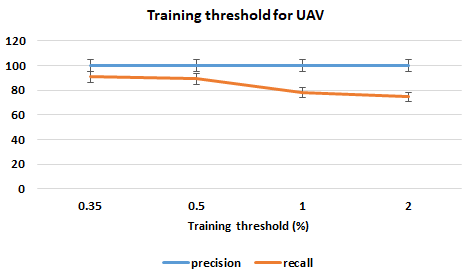
\includegraphics[scale=0.75,keepaspectratio = true]{Graphics/UAV_threshold.png}
    \caption{Result by varying the \textit{training threshold} for the UAV platform}
    \label{fig:UAV_threshold}
\end{figure}

\item \textit{Number of training traces}: By varying the training to testing traces ratio and keeping the training threshold at 0.5\%, we got the results described in ~\autoref{fig:UAV_traces}.
As can be observed, the number of training traces do affect the performance of \ac{CORGIDS}. Specifically, \ac{CORGIDS} achieve the best precision and recall when the training traces are maximum or near to the maximum value. Using 80\% or 70\% of the traces as training helped to achieve the recall of approximately 89 as opposed by lesser number of traces.

We see a dip in recall when the number of training traces decrease, because with fewer training data points, the \ac{HMM} does not get all the possibilities of the behavior that it can expect of the \ac{SUT}. Thus, more the number of training traces better the detection capability of \ac{CORGIDS}. Additionally, training the \ac{HMM} with different number of training traces did not make up a lot of time difference as compared to the experiment when the \textit{training threshold} was varied.

\begin{comment}
\begin{table}
\centering
  \caption{Result by varying the \textit{number of training traces} for the UAV platform}
  \label{tab:UAV_traces_results}
  \scalebox{0.9}{
  \begin{tabular}{|c|c|c|}
    \toprule
    \textbf{Number of training traces}&\textbf{Precision}&\textbf{Recall}\\
    \hline
    50\%: 50\% & 100.0 & 72.50\\
    \hline
    60\%: 40\% & 100.0 & 79.0\\
    \hline
    70\%: 30\% & 100.0 & 89.20\\
    \hline
    80\%: 20\% & 100.0 & 88.0\\
    \hline
\end{tabular}
}
\end{table}
\end{comment}

\begin{figure}[ht]
    \centering
    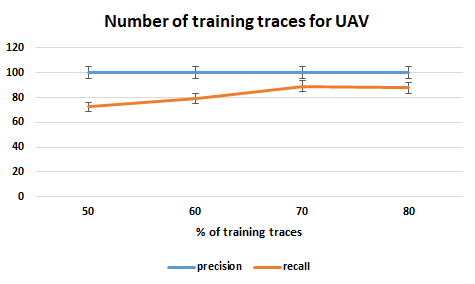
\includegraphics[scale=0.75,keepaspectratio = true]{Graphics/UAV_traces.png}
    \caption{Result by varying the \textit{number of training traces} for the UAV platform}
    \label{fig:UAV_traces}
\end{figure}

\end{itemize}

\subsection{Additional results for SAP platform}
We performed similar experiments for the training threshold and the number of training traces variables for the \ac{SAP} platform, with the results summarized below.

\begin{itemize}
\item \textit{Training threshold}: For this experiment, we used the same values of the training threshold from the above experiment involving the \ac{UAV} platform. That is, we varied the threshold between (0.35\%, 1.0\% and 2\%) with the experiments already conducted for the 0.5\% value in the attacks discussed in the ~\autoref{ch:Attacks}. The results are summarized in ~\autoref{fig:SAP_threshold}.

We see that the variation in the training threshold value has an effect on the recall of \ac{CORGIDS}. Particularly higher the value of training threshold, lower the recall of \ac{CORGIDS}, which means it is not able to detect malicious activities that well. However, the precision for all the experiments led to approximately similar value of 95. This could be because the HMM was able to capture the benign behavior of the \ac{SUT} with more precision. Further more, as the number of training traces for the \ac{SAP} platform were approximately 4 times less than the \ac{UAV} platform, it led to a very small number of training traces for each of the experiment conducted. Which is why the results of \ac{SAP} platform if compared with \ac{UAV} are lagging behind.

\begin{comment}
\begin{table}
\centering
  \caption{Result by varying the \textit{training threshold} for the SAP platform}
  \label{tab:SAP_threshold_results}
  \scalebox{0.9}{
  \begin{tabular}{|c|c|c|}
    \toprule
    \textbf{Training threshold}&\textbf{Precision}&\textbf{Recall}\\
    \hline
    0.35\% & 95.40 & 89.70\\
    \hline
    0.5\% & 95.70 & 93.70\\
    \hline
    1.0\% & 94.75 & 75.0\\
    \hline
    2.0\% & 95.30 & 57.50\\
    \hline
\end{tabular}
}
\end{table}
\end{comment}

\begin{figure}[ht]
    \centering
    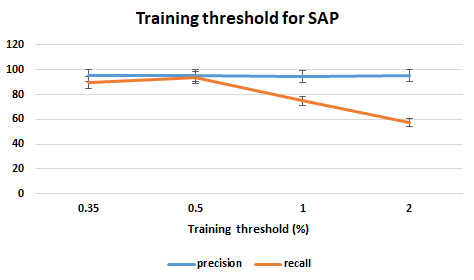
\includegraphics[scale=0.75,keepaspectratio = true]{Graphics/SAP_threshold.png}
    \caption{Result by varying the \textit{training threshold} for the SAP platform}
    \label{fig:SAP_threshold}
\end{figure}

\item \textit{Number of training traces}: By varying the ratio of training to testing traces and keeping the training threshold fixed at 0.5\%, we conducted experiments whose results are shown in~\autoref{fig:SAP_traces}. It is clearly seen that the number of training traces surely impacted the precision and recall of \ac{CORGIDS}. As anticipated, the few training traces led to less contextual behavior absorption for the \ac{HMM} which ultimately reflected on the evaluation metrics. For the attacks and result shared in ~\autoref{ch:Attacks}, we used 70\% : 30\% as the ratio and as can be seen from ~\autoref{fig:SAP_traces}, the precision and recall attained for these number of training traces achieve the maximum performance.

\begin{comment}
\begin{table}
\centering
  \caption{Result by varying the \textit{number of training traces} for the SAP platform}
  \label{tab:SAP_traces_results}
  \scalebox{0.9}{
  \begin{tabular}{|c|c|c|}
    \toprule
    \textbf{Number of training traces}&\textbf{Precision}&\textbf{Recall}\\
    \hline
    50\%: 50\% & 67.50 & 62.50\\
    \hline
    60\%: 40\% & 72.35 & 72.60\\
    \hline
    70\%: 30\% & 95.70 & 93.70\\
    \hline
    80\%: 20\% & 96.0 & 92.60\\
    \hline
\end{tabular}
}
\end{table}
\end{comment}

\begin{figure}[ht]
    \centering
    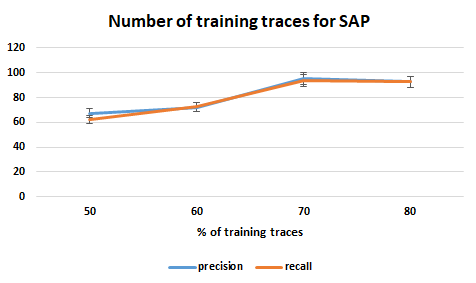
\includegraphics[scale=0.75,keepaspectratio = true]{Graphics/SAP_traces.png}
    \caption{Result by varying the \textit{number of training traces} for the SAP platform}
    \label{fig:SAP_traces}
\end{figure}

\end{itemize}

\section{Summary}

This chapter contains the results of sensitivity analysis which was performed to find out the values of three experimental factors which effected how the \ac{IDS} performed while detecting intrusion. It was found that as the window size increased and the acceptable range and threshold of consecutive decisions decreased, \ac{CORGIDS} performance was increasing, that is, fewer \ac{FP} and \ac{FN}. This observation was because the intrusion detector model uses \ac{HMM} and \ac{HMM} requires a slice of the current system trace for generating a result. If the slice of the trace will be small, it will lead to a narrow window of observations for the \ac{HMM}, thus not giving it enough data to analyze the current situation. Secondly, in this chapter we presented the results of prototyping \ac{CORGIDS} and using it for intrusion detection for the attacks mentioned in previous chapter. We use the two test-beds, an \ac{UAV} and a \ac{SAP} to prove that \ac{CORGIDS} is a generic IDS for \ac{CPS}. From the results we see that \ac{CORGIDS} achieve higher precision and recall as compared to the prior work. However, for \ac{SAP} the recall is less than ARTINALI due to lack of the system traces from which the \ac{IDS} was trained. Memory and performance overheads were also measured for the \ac{SAP} test-bed which indicated that \ac{CORGIDS} required approximately 36 MB of memory and took 1.25 seconds to generate a result - benign or malicious.

\endinput
=====================================================================
% EOF